
\chapter{Stellar spots cause measurable variations in atmospheric metallicity}
\label{chap:stellar_spots}

\section*{Preamble}

The effects of rotation can permeate astronomy in unexpected ways.
The number of stellar spots expressed by stars is directly tied to the surface rotation rate through increased magnetic field strength.
Stars with relatively fast rotation rates express larger surface spot coverage than those with slow rotation rates \citep{cao_starspots_2022}.
While stellar spots are useful in determining the surface rotation of stars, through periodic brightness variations, they have also been obtrusive in other areas.
For example, they can mimic transits of exoplanets in light curves.

In this work, we investigate the effect of stellar spots on the inferred atmospheric parameters of stars through spectroscopy.
We adopt a simple two-temperature model of the stellar atmosphere to reflect the impact of stellar spots on the stellar atmosphere.
With this model, we generate synthetic spotted spectra of a population of stars with physically motivated stellar and spot parameters
Then, we investigate the effect of fitting spotted spectra with non-spotted models of the stellar atmosphere.
We find that, even in this simple model of the impact of spots on the stellar atmosphere stellar spots can introduce bias and scatter to inferred atmospheric parameters.
The introduced scatter is particularly impactful to the precise measurement of stellar metallicity.


This chapter was originally published as:
\begin{quote}
	\citet{tanner_ss}
\end{quote}
and is presented in the form that it was published \update{in accordance with Monash University's thesis by submission guidelines.}



\newpage


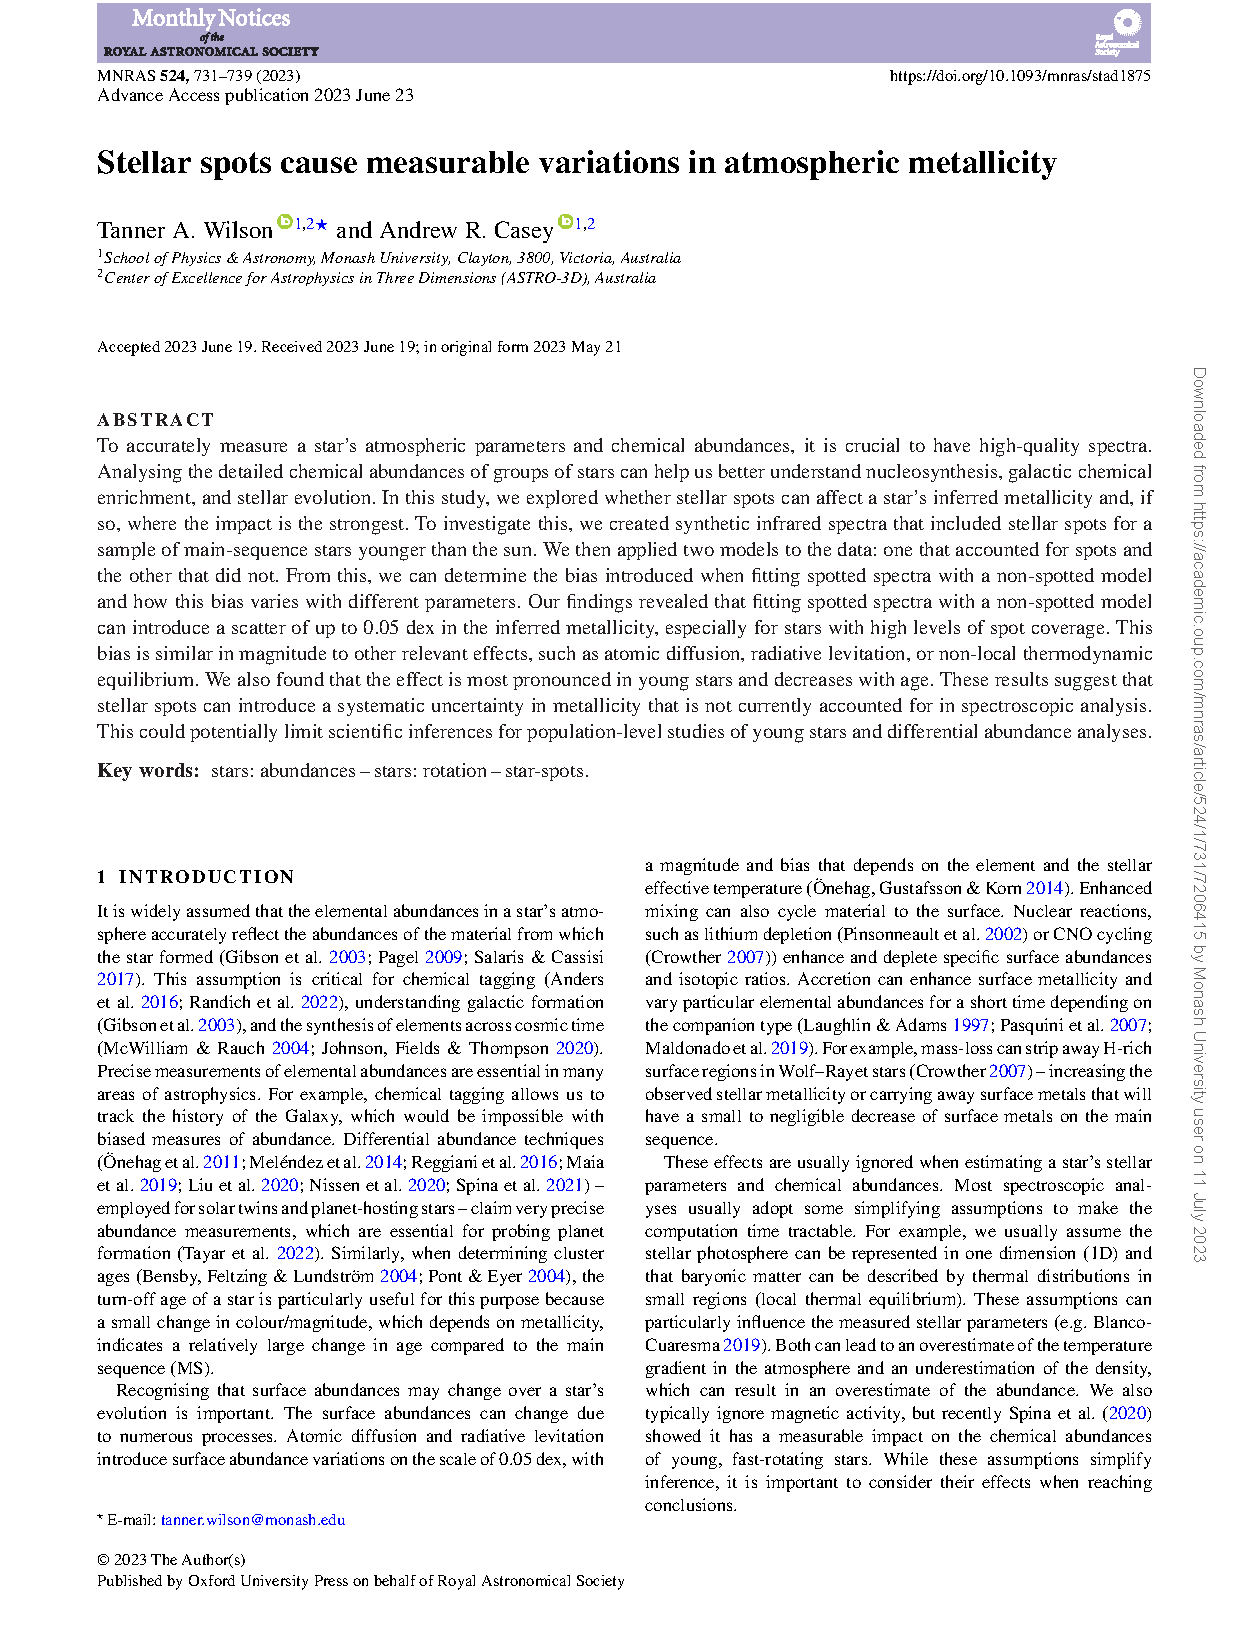
\includepdf[pages =1, addtotoc ={1,section,1, Introduction, p1}, scale=0.9,offset=65 -50]{Chapters/stad1875-TW-SS.pdf}


\includepdf[pages =2, addtotoc ={2,section,1, Method, p1, 2,subsection,2,Stellar parameters for a population of fake stars,p1},
addtolist = {2,figure,HR diagram of the 1500 sets of stellar parameters drawn from physically motivated distributions of mass{,} metallicity and age coloured by \feh.,f1}
, scale=0.9,offset=65 -50]{Chapters/stad1875-TW-SS.pdf}

\includepdf[pages =3, addtotoc ={3, subsection,2, Spotted spectrum generative model,p1},
addtolist = {3,figure,Recovered traditional stellar parameters (\teff{,} \logg{,} \feh \ and \vsini) from fitting synthetic spotted spectra with a spotted model of the stellar atmosphere against the corresponding injected parameters.,f1}
, scale=0.9,offset=65 -50]{Chapters/stad1875-TW-SS.pdf}

\includepdf[pages =4, addtotoc ={4,section,1, Results, p1},
addtolist = {4,figure,Recovered spot parameters from the synthetic spotted spectra fitted with a spotted model of the stellar spectra against the injected parameters of the synthetic spectra.,f1}
, scale=0.9,offset=65 -50]{Chapters/stad1875-TW-SS.pdf}

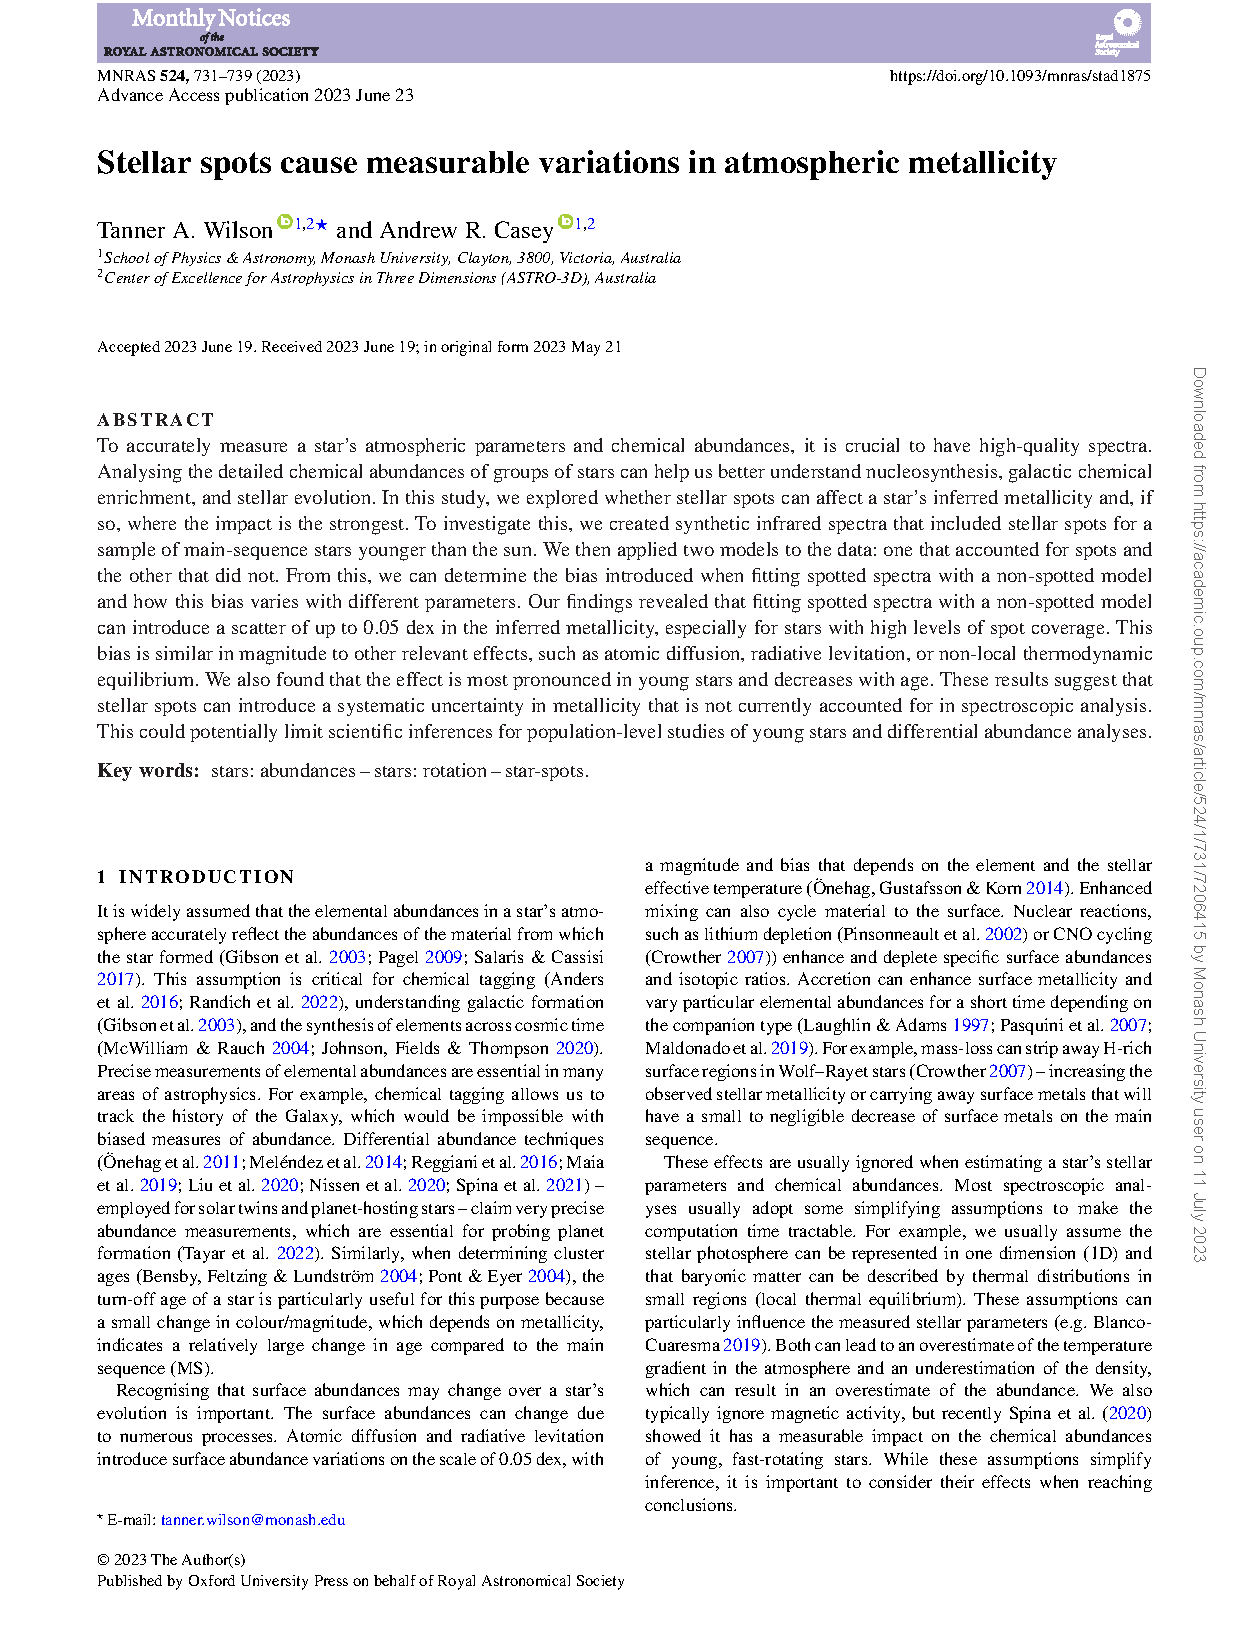
\includepdf[pages =5, addtotoc ={5,section,1, Discussion, p1, 5, subsection,2,Imperfect models,p1},
addtolist = {5,figure, The difference between the recovered traditional stellar spectra parameters (\teff{,} \ \logg{,} \ \feh \ and \vsini) from the synthetic spotted spectra fitted with both a spotted and non-spotted model of the stellar spectra against the injected parameters of the synthetic spectra.,f1}
, scale=0.9,offset=65 -50]{Chapters/stad1875-TW-SS.pdf}

\includepdf[pages =6,
addtolist = {6, figure, Bias introduced to \teff\ when fitting spotted spectra with a non-spotted model against injected parameters of synthetic spectra.,f1}
, scale=0.9,offset=65 -50]{Chapters/stad1875-TW-SS.pdf}

\includepdf[pages =7, addtotoc ={7, subsection,2,When should a spotted model of the stellar atmosphere be employed?,p1},
addtolist = {7,figure, Bias introduced to \logg  \ (orange){,} \feh \ (green) and $\log$ \vsini\ (red) when fitting spotted spectra with a non-spotted model against injected parameters of synthetic spectra.,f1}
, scale=0.9,offset=65 -50]{Chapters/stad1875-TW-SS.pdf}


\includepdf[pages =8, addtotoc ={8, section,1,Conclusions,p1},
addtolist = {8,figure, Bias introduced to \feh \ when fitting spotted spectra with a non-spotted model against the age of the model used to generate synthetic spectra.,f1}
, scale=0.9,offset=65 -50]{Chapters/stad1875-TW-SS.pdf}

\includepdf[pages =9, pagecommand={}, scale=0.9,offset=65 -50]{Chapters/stad1875-TW-SS.pdf}

